% !TEX root = ../main.tex
%\chapter{Background}
\chapter{Grundlagen}
\label{sect:basics}

In diesem Kapitel werden wir die, für die Entwicklung eines Frameworks im Bereich der Architekturvalidierung, notwendigen Konzepte und Technologien systematisch einführen. Zunächst gehen wir auf Middleware-Systeme in der Fahrzeugtechnik ein, wo wir deren Definition, typische Aufgaben sowie deren Bedeutung in der modernen Farhzeugtechnik zu erläutern. Basierend auf diesem Wissen folgt eine Darstellung der Software-Architekturen - inklusive eines Überblicks auf ASOA - in Bereich der Automobilindustrie: Wir beschreiben E/E-Architektur zudem diskutieren wir über die Rolle funktionaler und nicht-funktionaler Anforderung bei der Softwareentwicklung. Abschließend behandeln wir die Validierung dieser Architekturen, wobei sowohl die funktionale als auch ressourcenbezogenen Validierungsarten beleuchtet werden und die Relevanz der Automatisierung hierbei verdeutlicht wird.  

Diese Konzepte und Technologien bilden das Fundament für die anschließende Konzeption und Implementierung des Validierungs-Frameworks in den nachfolgenden Kapiteln

% Jedes Kapitel/Abschnitt sollte mit einem (zumindest kurzen) einführenden Text beginnen der 
% erklärt worum es in diesem Kapitel geht (siehe About Chapters and Sections)
% Each chapter should start with an (short) introduction explaining what the chapter is about 
% (see About Chapters and Sections)



% Die Abschnitte des Grundlagenkapitels sind exemplarisch!
% The sections of the fundamentals chapter are only examples!



\section{Middleware-Systeme in der Fahrzeugtechnik}
\label{sect:middleware}

Fahrzeuge haben sich seit dem ersten Serienauto (Benz Velo, 1894) (TODO:QUELLE), technologisch rasant weiterentwickelt. Ihre immer stärkere Vernetzung und Automatisierung erhöht die Systemkomplexität erheblich(TODO: QUELLE).Software-Middleware übernimmt hier zentrale Aufgaben, um Sensoren, Steueralgorithmen und Aktoren performant und zuverlässig zu verknüpfen.

Um zu verstehen, was Automotive Middleware ausmacht, beschäftigen wir uns zunächst mit den grundlegenden Konzepten der Middleware im Fahrzeugkontext. Die Hardware, welche in modernen Fahrzeugen zum einsatz kommen, werden durch die zugrunde liegende E/E-Architektur definiert.
\begin{definition}{E/E-Architektur}
	
\end{definition}

% ----------------------------------------------------------------------------------------------------

\section{Latex-technicals}
\label{sect:latex}

This section intends to introduce the reader without or only few latex knowledge to some basic latex commands.
It starts with a short introduction on how to get started with Latex and the setup of a latex environment.
In order to explain some useful features for document creation, Sect.~\ref{sect:citations} presents a citation command and gives some instructions on \textit{bibtex}.
Consequently, Sect.~\ref{sect:illustrations} explains how illustrations can be added to a document\footnote{A brief explanation on how to use symbols and abbreviations with this template can be found in appendix \ref{app:c}}.

\subsection{Setting up the environment}
\label{sect:latexenvironment}
The creation of documents using Latex can be compared to the creation of programs using a programming language like C.
This means that the Latex source files are simple text files.
These files describe the document being constructed and can be \enquote{compiled} to generate the document.
Accordingly a latex compiler is required by the user to create documents.
The open source project MiKTeX\footnote{\url{http://miktex.org/about}} includes such compilers.
This software-package contains everything needed to create Latex files out of this template.
Please note, that it does not contain all required packages to compile this document.
However, it is possible to obtain the required packages during latex compilation automatically.
If this is not initially the case, the feature can be enabled by starting the configuration program located at \enquote{Miktex install directory/miktex/bin/x64/mo\_admin}.
The option is configurable under the general tab at the section \enquote{package installation}.
Depending on the enabled/used features (e.\,g., creation of index etc.) this document requires to be created with additional parameters what can easily be done using the \texttt{compile.bat} script, delivered with this template.

As for programming languages \textit{Integrated Development Environments} (IDE) can support the user during his work.
An example for such an IDE compatible with MiKTeX is TeXnicCenter.
The reader might want to take a look at the correspondent website \url{http://www.texniccenter.org/}.


Since it has been explained how a Latex environment can be set up the following two sections describe some basic commands which will be needed to create scientific documents.

\subsection{Citations}
\label{sect:citations}

Latex is widely used to write scientific papers or theses.
A general commonality of such documents is the need to refer to work provided by other parties.
To cope with this need latex provides in combination with bibtex\footnote{bibtex is used to generate the bibliography} the \textbackslash cite\{reference-tag\} command.
During the creation of a latex document occurrences of the \textbackslash cite\{\} command are automatically replaced with squared brackets and a generated tag in between.
Those tags are listed in the bibliography with information about author, publisher, etc. referring to the literature information was taken from.
For instance, the command \textbackslash cite\{columbia\} will be transformed during creation of this latex document into \cite{columbia}.
This transformation requires that there is a correspondent entry for the \enquote{columbia} reference-tag in the \enquote{references.bib} file which comes with this latex template\footnote{In case a web content is referenced, a timestamp indicating the content was consulted shall be part of the bibliography entry. 
Moreover, offline copies of the contents need to be provided. This ensures that readers will be able to understand your work in the future when cited web content may have changed or be unavailable.}.

The next latex feature introduced in this document is the possibility to use illustrations, which is the topic of the following section.

\subsection{Illustrations}
\label{sect:illustrations}

Latex documents may contain pictures to support and visualize explanations.
They can be added to a document using the following commands:

\begin{flushleft}

\textbackslash begin\{figure\} \\
	\textbackslash centering \\
		\textbackslash includegraphics\{path\_to\_picture\} \\
	\textbackslash caption\{This caption will be shown below the figure\} \\
	\textbackslash label\{fig:label\_to\_referrence\_the\_figure\} \\
\textbackslash end\{figure\} \\

\end{flushleft}


An example how this looks after creation of the document is shown in Fig.~\ref{fig:logo}.
\begin{figure}[H]
	\centering
		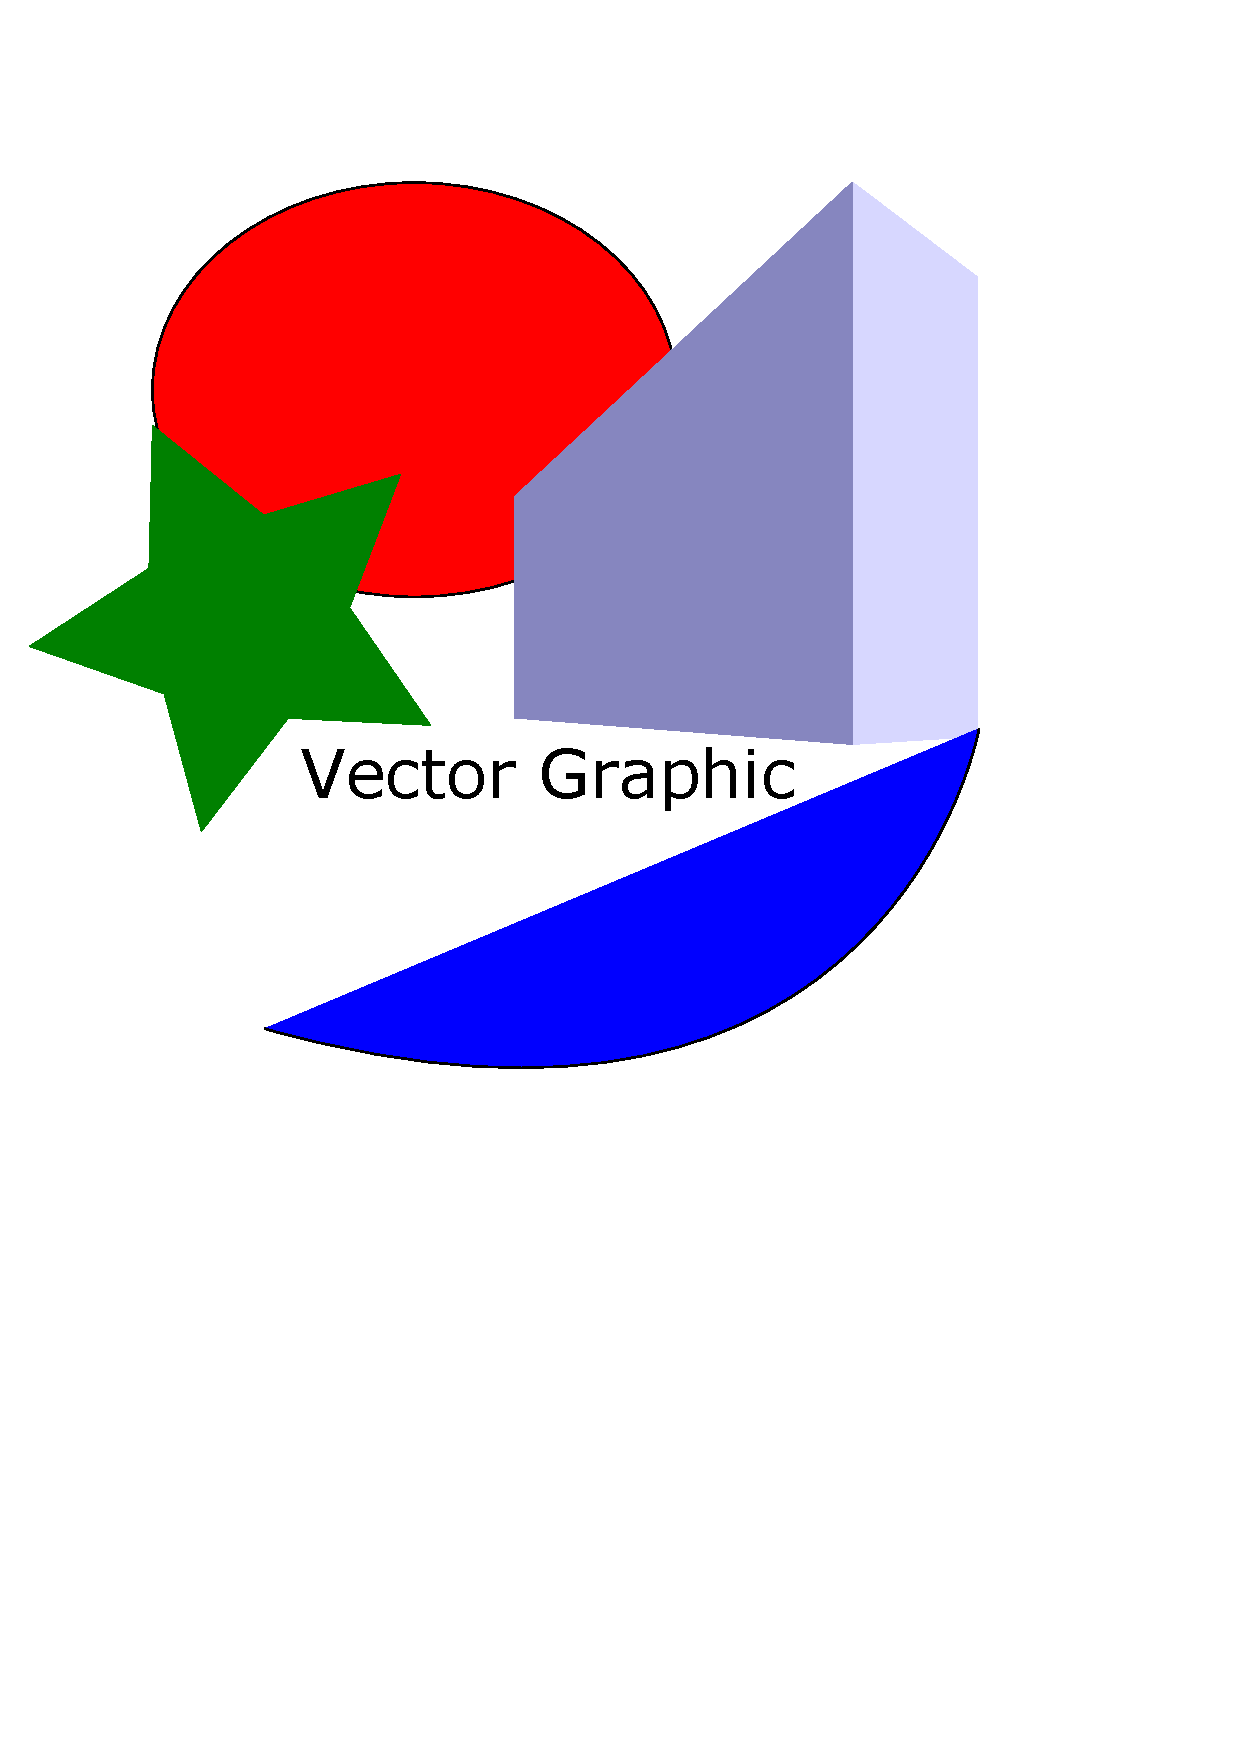
\includegraphics[width=0.40\textwidth]{figures/vectorGraphic.pdf}
	\caption{Example of a vector graphic}
	\label{fig:logo}
\end{figure}

Since this document is not the first and only one providing advice and hints regarding latex and structuring theses, the following chapter presents related work in this field.